The following chapter describes the build-up of the first two models, with regards to the use of libraries, agents, blocks and important variables and parameters. The structure of both models is divided into three parts: the waiting area, service lines and the inside of the airplane. The models contain three different types of agents, namely passengers, bins and seat blocks. These have been created in order to control key parts of the simulations, and will be described in more detail in the next section. Furthermore, the pedestrian library was used to simulate the passenger flow in the different sequences of the boarding process. 

\section{Model 1 - Boarding in Blocks}
The first model simulates a commonly used boarding strategy among airlines today, where passengers are called to board in groups, and within each group get on board in a random sequence. The model contains an excel-file, where 120 passenger IDs are assigned to specific seats, classes, boarding sequence, luggage quantity, colors, which bins to use and if the seat is located by the window, middle or aisle. The seating is divided into three groups (classes), which are passengers with special needs (seated in row 1), first class (seated in row 2-5) and economy class (seated in row 6-20). There are also "gold" passengers who don't have to get in line. The boarding sequence is prioritized in the following order: 1. Special needs, 2. First class/gold passenger, 3. Economy class back (row 12 - 20), 4. Economy class front (6 - 11). To keep track of the different groups while carrying out the simulation, passengers within each group are associated with a specific color. Special needs are red, first class blue, gold passengers golden and economy class green. 

\subsection{Airplane Layout}
The inside of the airplane consists of 120 seat nodes representing passengers seat locations. These are divided into 40 seat blocks and separates seats located on the left and right side of the aisle. There are 14 storage bins, where one bin is associated with 3 rows and has  a capacity of storing 9 luggage items. This applies for the first 12 bins, where the last 2 bins are associated with 2 rows.

\subsection{Passenger Source Block}
The model starts with a passenger source block, where 120 passengers are created and arrive at the waiting area with an arrival rate of 1 per second. This block assigns each passenger created with the data in the excel file. 

\subsection{Waiting Area}
When the passengers arrive in the waiting area they wait between 1 and 3 minutes. While they are waiting, the passengers are added to a collection in order to keep track of passengers waiting to board. Next, in the ped select output block the passengers are checking if they can board. This is based on a function where passengers are prioritized as described in the previous section. As long as the passengers with special needs have boarded, the rest of the passengers can start boarding if there are less than 8 people with higher priority in the boarding queue. If there are more than 8 people in the queue, they will wait between 5 and 20 seconds before checking again.   

\subsection{Service Area}
The ped service block is visualized through a single queue where passengers have to show their documentation in order to board the plane. Passengers who exit the queue are removed from the collection containing passengers waiting to board, which enables passengers with lower priority to start boarding. Then they start moving towards the start of the aisle inside the plane.

\subsection{Storing Luggage}
When passengers arrive at the start of the seat rows, they first go to the bin location associated with their seat block. The luggage storing process is represented through the check bin block, where passengers who do not have any luggage can proceed to sit down in their seats. If the passenger has luggage and there is available space in the bin, the luggage will be stored and the passenger is then seated. In the case where the bin is full, the passenger will check the nearest bins. If there is available space, they will store their luggage there and go to their seats. 

\indent\newline
In order to make passengers stop and wait for others who are storing luggage, the passengers who are storing luggage checks who is in front of them and who is behind them, and is then added to two collections. This is done by calculating the distance between the passenger checking, and other surrounding passengers within a certain range. A negative distance means that the passengers are located behind, while a positive distance means that passengers within the range are in front of the passenger checking. If a passenger has someone in front of them storing luggage, they will slow down their walking speed, move up towards them, but not pass them. A limitation in the model is that it does not account for a situation where the total bin capacity is exceeded. On the other hand, this can sometimes be resolved by storing some of the luggage beneath the seats.   

\subsection{Letting Passengers get to their Seats}
An important part of the boarding process is to simulate passengers getting up from their seats to let another passenger in. A combination of a ped select output block and two ped wait blocks is used to do this. If there are passengers already seated in the row, and if they are interfering with the passenger trying to get to his or her seat, they will get up from their seats and move into the aisle.  

\subsection{Colors}
There are several variables (constants) regarding colors included in the model. The purpose is to help visualize different states in the model. When passengers are storing luggage, the color of the passengers turn pink, and when they are searching for another bin the color changes to purple. In situations where they have to get up from their seats to let another passenger in, they turn violet. Finally, when passengers are seated they change color to white.    

\section{Model 2 - Steffen's Method}
The second model is a boarding method proposed by Steffen J. who is a researcher on boarding problems. The method involves passengers being called to board the plane in a given sequence. The boarding sequence works as follows: The first passenger called to board is seated at the last row by the window on the right side of the aisle. Then the second passenger is also seated at the right side by the window, but two rows before the first passenger. The process continues for one side of the plane and is repeated on the other side, again starting with the window seats. In summary, the window seats are filled up first, then the middle and lastly the seats in the aisle:

\begin{table}[H]
  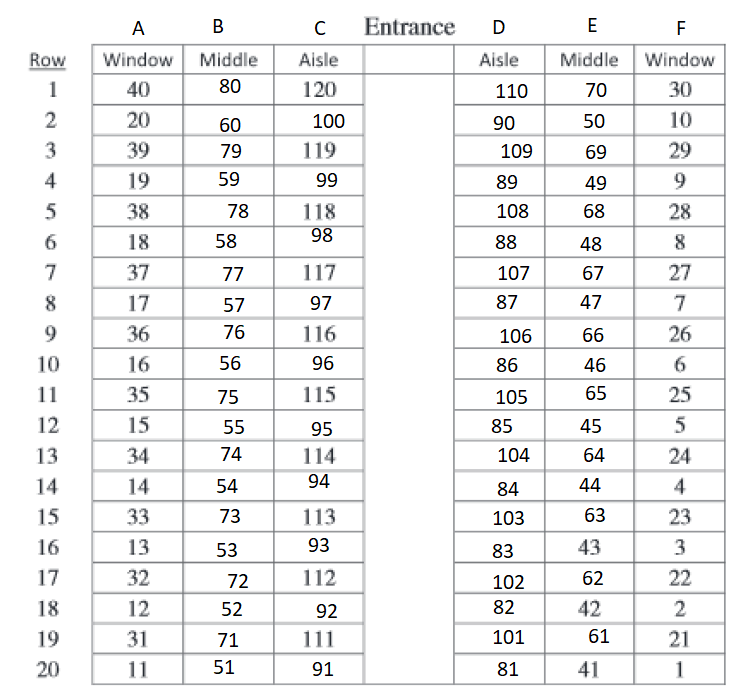
\includegraphics[width=0.75\textwidth]{tables/table1.png}
  \caption{Steffen's Method}
  \label{tbl:table1}
\end{table}

The structure of the model is based on the same logic as in the first model, which means that it consists of a waiting area, service area and the inside of the plane. However, there are some elements different from the first model, which will be explained next.

\subsection{Data from the Excel-File}
The passenger IDs in the excel-file are associated with a different seat location, and represent the specific boarding sequence as proposed by Steffen J. This means that passenger ID 1 is given seat number 20F, passenger ID 2 is given seat number 18 F etc. The model does not take into consideration the different groups of passengers (classes) and is visualized through all of the passengers having the same color.

\subsection{Service Area}
The queue to the boarding service is constructed as a serpentine queue, opposed to the service queue in the first model. The reasoning behind this is to avoid a situation where there are passengers entering the plane before everyone is present in the waiting area. Another reason is to create a longer queue, so the airport employees can make sure that the passengers are boarding in the correct order. Since the two models differ in this part, it will be taken into consideration when comparing the time measurement between the models. 

